\chapter{Memory Virtualization}

\section{The Abstraction: Address Space}

\textbf{Address Space: The running program's view of memory in the system}\\

\begin{tcolorbox}
    \begin{center}
        \textbf{The Crux: How to Virtualize Memory?}
    \end{center}

    How can the OS build this abstraction of a provate, potentially large
    address space for multiple running processes (all sharing memory) on 
    top of a single, physical memoty?
\end{tcolorbox}

Goals of OS while virtualizing memory:

\begin{enumerate}
    \item Transparency: How OS implements virtual memory should be invisible
        to the running program.
    \item Efficiency
    \item Protection: A process should not be able to access memory out of
        its virtual memory
\end{enumerate}

\section{Mechanisms}

\begin{tcolorbox}
    \begin{center}
        \textbf{The Crux: How to Efficiently And Flexibly Virtualize Memory}
    \end{center}

    How can we build an efficent virtualization of memory? How do we maintain
    control over the locations application can access? how do we do all of
    this efficently?
\end{tcolorbox}

How it will work:

\begin{itemize}
    \item Hardware provides mechanisms for \textbf{hardware-based address
        translation}. Hardware only provides the low-level mechanisms.
    \item OS will use these mechanisms to manage memory, keeping track of free
        memory and maintain control.
\end{itemize}

Assumptions we make for now:

\begin{itemize}
    \item Address space must be placed \textit{contiguously} in physical
        memory.
    \item Size of address space is less than size of physical memory.
\end{itemize}

We will continue to relax these assumptions as we develop a better model. The
current model will be laughable at best.\\

What the process should see:

\begin{figure}[h!]
    \begin{center}
        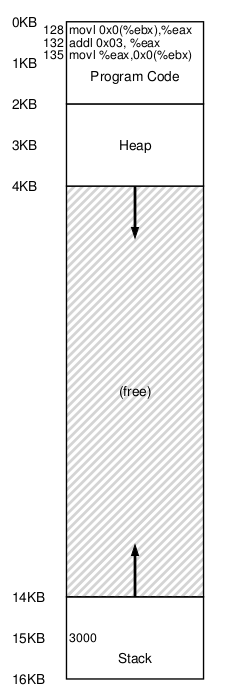
\includegraphics[width=4cm, height=6cm]{img/151.png}
        \caption{A process and its address space}
    \end{center}
\end{figure}

What should actually go in memory:

\begin{figure}[h!]
    \begin{center}
        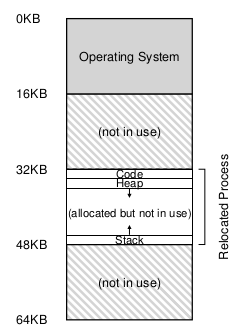
\includegraphics[width=4cm]{img/152.png}
        \caption{Physical Memory with the process}
        \label{152}
    \end{center}
\end{figure}

The program thinks its address space starts at address 0, while it actually
starts at 32KB in the physical memory.

\subsection{Dynamic(Hardware-based) Relocation}

We discuss the furst incarnation of address translation:
\textbf{base and bounds}.\\

Specifically, we'll need two hardware registers within each CPU: one called
the \textbf{base} register, and the other the \textbf{bounds} register. Using
base and bounds, we can place the address space anywhere we like in the 
physical memory and ensure that it only has access to its own address space.\\

In this setup, each program is written and compiled as if it is loaded at
address zero. However, when running the OS decides where in physical memory
to place the program and sets the base register to that value. Now, the 
physical address can be calculated as:

$$
physical\ address = virtual\ address + base
$$

Memory refrences generated by the process are \textbf{virtual addresses}. The
hardware turns these virtual addresses into \textbf{physical addresses}.
This technique of transforming a virtual address is exactly what is refered as
\textbf{address translation}
The bounds register is used to check if the virtual address lies in the virtual
memory or not.\\

Since this relocation happens at runtime and we can move address spaces after
process has started runnning, this technique is reffered to as \textbf{dynamic
relocation}\\

Note that base and bounds registers are hardware structures kep on the CPU
chip. This part of processor which helps with address translation is called
\textbf{Memory Management Unit (MMU)}. We will continue to add more circuity
to MMU.\\

\paragraph{Hardware Support Summary till now}

\begin{itemize}
    \item \textbf{Privileged mode}: Needed to prevent user-mode processes 
        from executing privileged instructions
    \item \textbf{Base/bounds registers}: pair of registers per CPU to support
        address translation and bound checks
    \item \textbf{Privileged instructions to update base/bounds}
    \item \textbf{Privileged instructions to register exception handlers}: How
        to handle exceptions must be told by the OS
    \item \textbf{Ability to raise exceptions}
\end{itemize}

\paragraph{OS Requirement Summary for memory}

\begin{itemize}
    \item \textbf{Memory Management}: Need to allocate memory for new processes,
        reclaim memory from terminated processes, manage memory via \textbf{free
        list}.
    \item \textbf{Base/bounds management}: Must set base/bounds properly
        upon context switch.
    \item \textbf{Exception handling}: Code to run when exceptions arise.
\end{itemize}

Base and bounds virtualization is quite \textit{efficient} but it has a
\textbf{lot} of problems. As can be seen in Figure \ref{152} all of the space
between the stack and heap is wasted. This is called
\textbf{internal fragmentation}.

\subsection{Segmentation}

\begin{tcolorbox}
    \begin{center}
        \textbf{The Crux: How To Support A Large Address Space}
    \end{center}

    How do we support a large address space with (potentially) a lot of free 
    space between the stack and heap?
\end{tcolorbox}

Basic idea $\rightarrow$ \textbf{Segmentation}. Instead of having just one base
and bounds pair in our MMU, why not have a base and bounds pair per logical
segment of the address space? In our address space, we have three
logically-different segments: code, stack, and heap. In segmentation, we place
each one of those segments in different parts of memory.

\subsubsection{Which Segment Are We Referring To?}

Two approaches:

\begin{enumerate}
    \item \textbf{Explicit} approach: Chop up the address space into segments
        based on few bits of the virtual address.

        \begin{figure}[h!]
            \begin{center}
                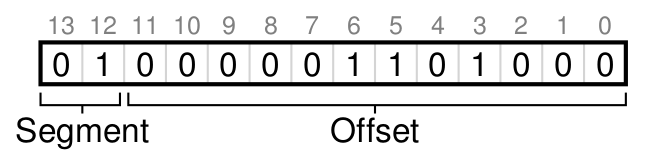
\includegraphics[width=4cm]{img/explicit.png}
                \caption{Chopping virtual address}
            \end{center}
        \end{figure}
    \item \textbf{Implicity} approach: The hardware determines the segment by
        noticing how the address was formed.
\end{enumerate}

Since out memory can grow forward or backward, we add another piece of
information in hardware that wether the segment grows positively or negatively.

\subsubsection{Support for Sharing}

To save memory, sometimes it is useful to \textbf{share} certain memory
segments between address spaces. In particular, \textbf{code sharing} is common
nowdays.\\

To support this, we need to add more support for hardware in form of
\textbf{protection bits}. Basic support adds a few bits per segment, indicating
read/write/execute permissions. Trying to do something out of permission should
raise an exception.

\subsubsection{OS Support}

\begin{enumerate}
    \item The OS has to save all base and bound register when a context
        switch occurs.
    \item OS interaction when segments grow: if malloc() os called, in some
        cases the heap may be able to service the object. If it can, find
        free space for the object and return a pointer to it. If the heap
        needs to grow, call a system call to grow the heap.
    \item Managing free space: When a new address is created, the OS has to be
        able to find space in physical memory for its segments. The general
        problem that arises is that physical memory soon becomes full of holes 
        and to allocate a contigous block of memory, you will have to move some
        blocks around. This problem is called \textbf{external fragmentation}.
\end{enumerate}

The main problem right now is using a varibable sized chunks.

\section{Paging}

Chop up space into \textit{fixed-size} pieces $\rightarrow$ \textbf{paging}\\

\begin{tcolorbox}
    \textbf{The Curx: How To Virtualize Memory With Pages}

    How can we virtualize memory with pages, so as to avoid the problems 
    faced by segmentation? What are the techniques and how do we make them work
    efficently?
\end{tcolorbox}

Paging, has a number of advantages over our previous approaches:

\begin{itemize}
    \item Probably the most important improvement will be \textit{flexibility}:
        with a fully-developed pagin approach, the system will be able to 
        support the abstraction of an address space effectively, regardless
        of how a process uses the address space. For example, no assumptions
        in the way stack and heap grow.
    \item Another advantage is the \textit{simplicity} of free-space management
        that paging affords. For example, when the OS wishes to allocate lets
        say 64-byte address space into the physical memory, it just finds
        four free pages for this. OS keeps some kind of \textbf{free list}
        of all free pages for this.
\end{itemize}

To record where each virtual page of the address space is placed in physical 
memory, the operating system usually keeps a \textit{per-process} data 
structure known as \textbf{page table}. The major role of the page table is
to store \textbf{address translations} for each of the virtual pages of the
address space, thus letting us know where in physical memory each page
resides.\\

The page table is a \textit{per-process} data structure (most page table
structures we do here are like this, an exception is \textbf{inverted page
table}). If another process wanted to run, we would have to change our page
table.\\

\subsection{Virtual Address Translation}

Let's imagine the process with a tiny address space (64 bytes) is performing
a memory access:

\begin{lstlisting}
    movl <virtual address>, \%eax
\end{lstlisting}

To \textbf{translate} this virtual address that the process generated, we have
to first split it into two components: the \textbf{virtual page number (VPN)},
abd the \textbf{offset} within this page. For this example, we need need 6 bits
total as $2^6 = 64$. Because we know the page size (16 bytes), we divide the
virtual address as follows:

\begin{figure}[h!]
    \begin{center}
        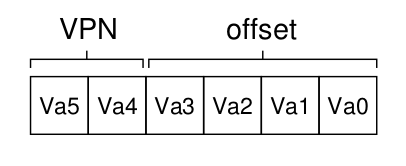
\includegraphics[width=4cm]{img/vapage.png}
        \caption{Virtual Address of the example}
    \end{center}
\end{figure}

Lets say that we have out virtual address as $21$, the VPN is $01$,
lets say it maps to the
$7^{th}$ \textbf{physical frame number (PFN)} also called the \textbf{physical
page number (PPM)}. Thus we can translate this address by replacing the VPN
with the PFN and then issue the load to physical memory.

\begin{figure}[h!]
    \begin{center}
        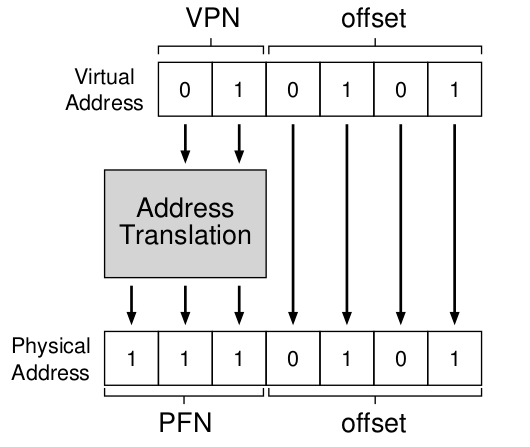
\includegraphics[width=5cm]{img/183.png}
        \caption{The Address Translation Process}
    \end{center}
\end{figure}

Note that the offset stays the same, because the offset just tells us which
byte \textit{within} the page we want.

\subsection{Where Are Page Tables Stored?}

Page tables can get terribly large, much bigger than the small segment table
or base/bounds pair we discussed previously. For example, for a 32-bit address
space, with 4KB pages, we have a 20-bit VPN and 12-bit offset. A 20-bit VPN
implies that there are $2^20$ translations that the OS would have to manage
for each process. Assuming we need 4 bytes per \textbf{page table entry (PTE)}
to hold the physical translation plus any other useful info, we get 4MB of 
memory needed for each page table, i.e. we need 4MB for each process. If we
have a 100 processes running at a time, the Page Tables are using 400MB, which
is too much. This will be even worse for 64-bit address space. Since they are
so big, we dont keep any special onchip-hardware in MMU to store. We store it
in the memory.

\subsection{What is in the Page Table?}

The page table is just a data structure used to map virtual addresses to
physical addresses. For now, we use a \textbf{linear page table}, which is
just an array. Later we'll use more complex structures to reduce memory.\\

We add the following things to a PTE:

\begin{enumerate}
    \item A \textbf{valid bit} to indicate if the particular translation is
        valid. For example, on a running code we have stack and heap on 
        opposite ends. The space inbetween them will be invalid. Accessing 
        invalid positions will generate a trap to OS which will say
        \text{GOODBYE OFFENDING PROCESS}.
    \item \textbf{protection bits} indicating read/write/execute permissions.
    \item A \textbf{present bit} indicates wether this page is \textbf{swapped
        out} (Will study this further)
    \item A \textbf{dirty bit} indicating if the page has been modified since
        the last time it was brought into memory.
    \item \textbf{reference bit} Useful in determining which pages are popular.
        Such knowledge is critical during \textbf{page replacement} (Further)
\end{enumerate}

\begin{figure}[h!]
    \begin{center}
        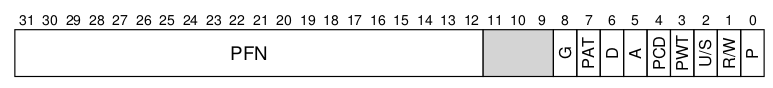
\includegraphics[width=6cm]{img/185.png}
        \caption{An x86 Page Table Entry (PTE)}
    \end{center}
\end{figure}

\subsection{Paging: Also Too Slow} 

The OS first goes to the memory and looks at the page table, brings back the 
translation, then again goes to memory to access the physical address mapped
to the virtual address. Here is code for how it is done:

\begin{figure}[h!]
    \begin{center}
        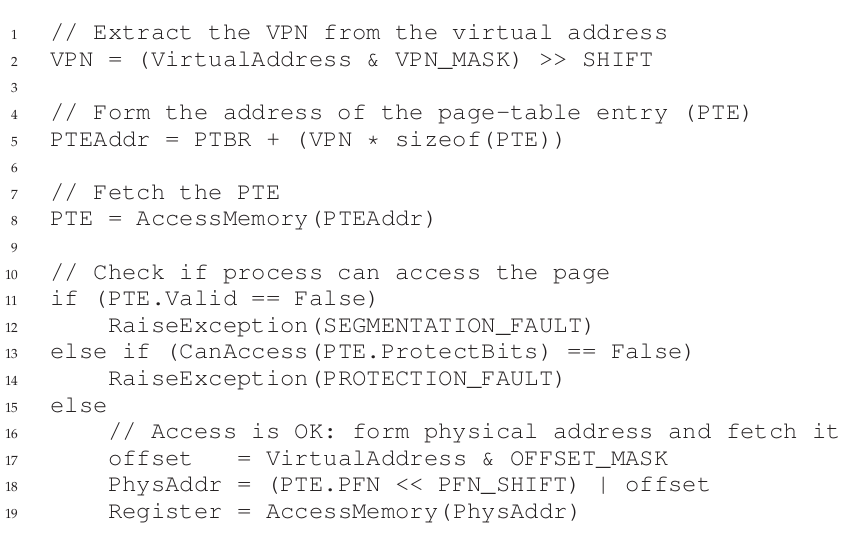
\includegraphics[width=8cm]{img/186.png}
        \caption{Accessing Memory with Paging}
    \end{center}
\end{figure}

We have extra memory references which likely slow down the process by a factor
of two or more.

Problem with paging $\rightarrow$ if not designed carefully, it will cause the
system to run too slow as well as take too much memory. We need to overcome 
these two problems now.

\subsection{Faster Translations (TLBs)}

\begin{tcolorbox}
    \begin{center}
        \textbf{The Crux: How To Speed Up Address Translation}
    \end{center}

    How can we speed up address translation, and generally avoid the extra
    memory refernce that paging seems to require? What hardware support is
    required? What OS involvement is needed? 
\end{tcolorbox}

To speed up address translation, we are going to add \textbf{translation-
lookaside buffer or TLB}. A TLB is part of the chip's \textbf{memory-
management unit (MMU)}. It is basically \textbf{cache} for popular
virtual-to-physical translations.\\

The algorithm hardware follows is like this:

\begin{itemize}
    \item Extract the VPN from virtual address
    \item If the VPN is present in the TLB then it is a \textbf{TLB hit}.
        Extract the PFN and concatenate it with the offset.
    \item If it is a \textbf{TLB miss}, hardware accesses the page table
        to find the translation, assuming that the virtual reference generated
        by the process is valid and accessible, updates the TLB with the
        translation. A TLB miss is expensive because of the extra memory
        reference.
    \item Finally, once the translation is found in the TLB, the memory 
        reference is processed quickly.
\end{itemize}

The TLB like all caches is based on spatial and temporal locality.

\subsubsection{Who Handles The TLB Miss?}

TLB miss can be handled by the hardware or the OS.\\

In the olden days, the hardware had \textbf{CISC} architecutre and handled the
TLB miss entirely. To do this, the hardware has to know exactly \textit{where}
the page tables are located in memory as well as their \textit{exact format}.
On a miss, the hardware would find the page-table entry and extract the
desired translation, update the TLB with the translation and retry the
instruction. Intel x86 architecture uses \textbf{hardware-managed page TLBs} 
with a fixed \textbf{multi-level page table} (will study further)\\

More modern architectures with \textbf{RISC} style have what is
known as a \textbf{software-managed TLB}. On a TLB miss, the hardware simple 
raises an exception, which pauses the current instruction stream, raises the
privilege level to kernal mode and jumps to a \textbf{trap handler}. The
trap handler handles the miss. Main reason of using OS to handle miss is 
more \textit{flexibility}.

\subsubsection{TLB Contents}

A TLB has working similar to cache. But what is the data in it? A TLB entry
might look like this:

\begin{center}
    VPN $|$ PFN $|$ other bits
\end{center}

The interesting part is the "other bits". For example, the TLB commonly has a
\textbf{valid} bit,  which says wether the entry has a valid translation or
not. Also common are \textbf{protection} bits, which determine the permissions
the process has for the memory. There might be other fields, including an
\textbf{address-space indentifier}, a \textbf{dirty bit}, and so forth.

\subsubsection{Context switches with TLB}

\begin{tcolorbox}
    \begin{center}
        \textbf{The Crux: How To Manage TLB Contents On A Context Switch}
    \end{center}

    When context-switching between processes, the translations in the TLB
    for the last process are not meaningful to the about-to-be-run process.
    What should the hardware or OS do in order to solve this problem?
\end{tcolorbox}

One way would be to flush the TLB on context switches, thus emptying it before
running the new process. However this is costly if the processes are switched
frequently.\\

To reduce this overhead, some systems add hardware support to enable sharing of
the TLB across context switches. In particular some systems provide an
\textbf{address space identifier (ASID)} field in the TLB which can be thought
of as a \textbf{process indentifier (PID)}, but usually takes fewer bits. Here
is a depiction of TLB with the added ASID field:

\begin{figure}[h!]
    \begin{center}
        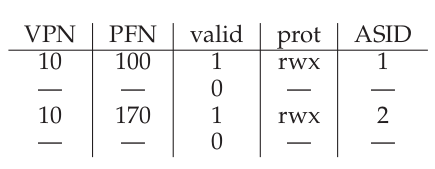
\includegraphics[width=5cm]{img/ASID.png}
        \caption{TLD entry with ASID}
    \end{center}
\end{figure}

Now the TLB can hold translations from different processes at the same time
without any confusion. The hardware also needs to know which process is
currently running in order to perform translations, and thus the OS must, on 
a context switch, set some privileged register to the ASID of the current
process.

\subsubsection{Replacement Policy}

The replacement policies are same as \textbf{cache replacement}. Duh, its a
cache. What were you expecting? Anyway, this part is covered in swapping.

\subsection{Paging: Smaller Tables}

\begin{tcolorbox}
    \begin{center}
        \textbf{The Crux: How To Make Page Tables Smaller}
    \end{center}

    Simple array-based page tables are too big. How can we make page tables
    smaller? What are the key ideas? What inefficiencies arise as a result of
    these new data structures?
\end{tcolorbox}

Some solutions with their problems:

\begin{itemize}
    \item \textbf{Bigger Pages:} Can lead to internal fragmentation due to
        pages not being used completly.
    \item \textbf{Paging + Segments}: Divide segments into pages. Doesnt really
        solve the main problem of segmentation i.e. external fragmentation.
\end{itemize}

\subsubsection{Multi-level Page Tables}

Get rid of all the invalid regions in the page table instead of keeping them
all in memory.\\

We turn the linear page table into something like a tree. The basic idea is 
simple, chop up the apge table into page-sized units; then if an entire page of
page-table entries (PTEs) is invalid, dont allocate that page of the page table
at all. To track wether a page of the page table is valid, use a new structure
called the \textbf{page directory}. the page tells you where a page of the
page table is or that the entire page of the page table contains no
vali pages.

\begin{figure}[h!]
    \begin{center}
        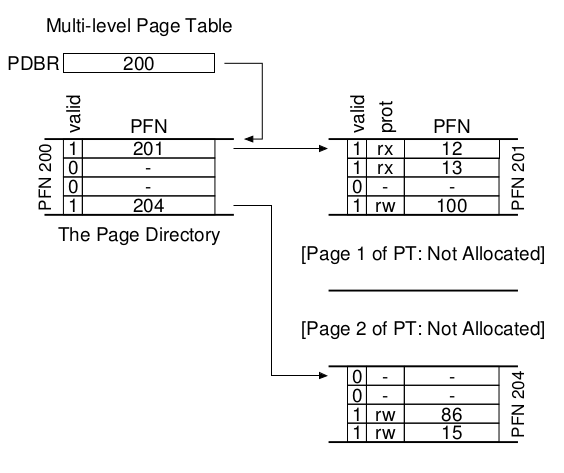
\includegraphics[width=5cm]{img/203.png}
        \caption{2-Level Page Table}
    \end{center}
\end{figure}

Advantages of Multi-level page tables:

\begin{itemize}
    \item They only allocate page-table space in proportion to the amount of
        address space you are using; thus it is good for sparse address
        spaces
    \item If carefully constructed, each portion fits neatly within a page,
        making it easier to manage memory.
\end{itemize}

It should be noted that there is a cost to multi-level tables; for the
2-level page table, we required two loads from memory to get the right
translation information from the page table (one for the page directory and
one for the PTE itself). Smaller tables 
give higher TLB miss cost but reduce space.
This is a space-time tradeoff. The cost in a TLB hit is the same.\\

We dont have to use only 2-level page tables. For larger physical memory, 
we need to use higher level page tables to get smaller tables. We create a
page directory of page directories and so on. Levels can be decided based on
how much reduction we need.\\

New code for Address translation:

\begin{figure}[h!]
    \begin{center}
        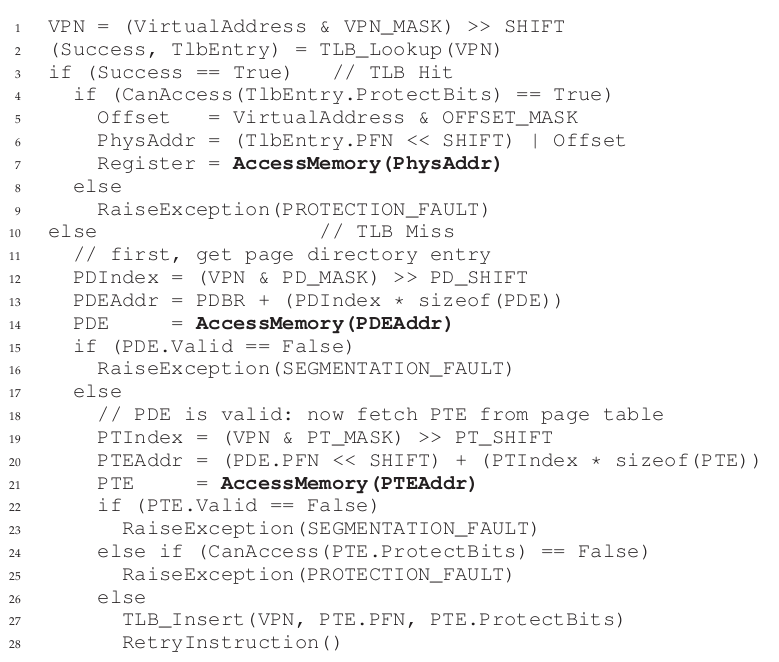
\includegraphics[width=7cm]{img/206.png}
        \caption{Mutli-level Page Table Control Flow}
    \end{center}
\end{figure}

As it can be seen, only the cost of TLB miss has been increased and not that
of a TLB miss.


\section{Swapping}

Now we relax the assumption that our address space is unrealistically small
and fits into physical memory,

\begin{tcolorbox}
    \begin{center}
        \textbf{The Crux: How To Go Beyond Physical Memory}
    \end{center}

    How can the OS make use of a larger, slower device to transparently provide
    the illusion of a large virtual address space?
\end{tcolorbox}

First, we need to reserve some space for swaping. we generally refer to such
space as \textbf{swap space}. Thus, we simply assume that the OS can read from
and write to the swap space, in page-sized units. OS needs to remember the
\textbf{disk address} of a given page to accomplish this.\\

Now that we have some space on disk for swapping, we need to add machinery in
the system to support swapping pages to and from the disk. We assume that we
have a system with a hardware-managed TLB (like x86 has).\\

We need to add more machinery to the \textbf{page table entry (PTE)}. It must
now have a \textbf{preset bit}, which indicates wether the page is in memory.
In the case that the hardware looks in the TLB and the page is \textit{not
present}, the OS is invoked to service the \textbf{page fault}. The handler
invoked is called \textbf{page-fault handler}. It runs and services the page
fault.\\

When the OS receives a page fault for a page, it looks in the PTE to find the
address, and request to disk to fetch page into memory. When disk I/O completes
, the OS will then update the page table to mark the page as present, update
the PFN field of the page-entry (PTE) to record the in-memory location of
the newly-fetched page, and retry the instruction. While the I/O is in flight, 
the process will be blocked and the OS is free to execute other processes.\\

In the process above, if the memory is full then we use a \textbf{page
replacement policy} to kick out, or replace pages from memory.
